\documentclass[12pt,a4paper]{article}
\usepackage{placeins}
\usepackage[utf8]{inputenc}
\usepackage[ruled]{algorithm2e}
\usepackage{fullpage}
\usepackage{graphicx}
\usepackage{float}
\usepackage[portuguese]{babel}
\usepackage[]{amsmath}
\restylefloat{figure}

\usepackage[adobe-utopia]{mathdesign}
\usepackage[T1]{fontenc}

% \usepackage{mdframed}

\DeclareGraphicsExtensions{.jpg,.pdf}

\numberwithin{equation}{section}

\title{Trabalho Prático 4 - Ligador}
\author{Victor Pires Diniz}

\begin{document}
\maketitle
\begin{center}
Software Básico - 2º Semestre de 2015
\end{center}

\section{Descrição do trabalho}

O terceiro trabalho prático do semestre envolve o desenvolvimento de um ligador para o código de máquina de uma máquina virtual especificada, para a qual foram feitos um emulador, um expansor de macros e um montador nos três trabalhos prévios. O ligador permite a modularização dos programas no assembly da máquina, permitindo a expansão de macros e montagem separada de cada módulo e conectando o código de máquina gerado pelos módulos em um só arquivo, que pode ser executado pelo emulador.

O ligador proposto na especificação deveria ser capaz de ligar os sub-programas com base em informação extra sobre os símbolos de cada módulo fornecida durante o processo de montagem. Por essa razão, foi necessário realizar algumas mudanças também no montador, para que esse pudesse imprimir a tabela de símbolos dos módulos antes do programa.

\section{Implementação e decisões de projeto}

O código do ligador está dividido semanticamente entre vários módulos:

\begin{itemize}
    \item \emph{main.c}: recebe parâmetros por linha de comando e chama o ligador apropriadamente.
    \item Map (\emph{map.c, map.h, bucket.c, bucket.h}): implementa uma tabela de dispersão genérica, instanciada na tabela de macros.
    \item Função hash auxiliar (\emph{hash\_aux.c, hash\_aux.h}): contém uma função para hashing de string.
    \item Funções auxiliares para strings (\emph{str\_aux.c, str\_aux.h}): contém duas funções para auxiliar no uso de strings ao longo do código.
    \item Vector (\emph{vector.c, vector.h}): implementa uma lista dinâmica de tipo único, utilizada na implementação do ligador para agregar os módulos.
    \item Tabela de símbolos (\emph{sym\_table.c, sym\_table.h}): tipo implementado para contenção da tabela de símbolos de cada módulo carregado. Usa a biblioteca \emph{Map} internamente.
    \item Ligador (\emph{linker.c, linker.h}): módulo principal do ligador. Define a função principal do programa e, internamente, realiza as duas passadas do ligador.
\end{itemize}

Os mais importantes deles serão analisados a seguir em mais detalhe.

\subsection{Map}

O módulo map contém a implementação de uma hash table totalmente genérica, com tratamento de colisão através de listas encadeadas, definidas nos arquivos \emph{bucket.c} e \emph{bucket.h}.

\subsection{Vector}

Este módulo implementa uma lista genérica dinamicamente alocada para armazenar as linhas de código de montagem das macros. A implementação dessa lista é feita de maneira contígua, com um vetor interno à estrutura. Esse vetor é expandido dinamicamente conforme necessário, crescendo exponencialmente (por um fator de 1,5) sempre que o número de elementos alcança o número máximo de elementos do vetor.

\subsection{Tabela de símbolos}

Define um tipo abstrato de dados para ser utilizado como tabela de símbolos, criando uma camada de abstração sobre um Map e escondendo os detalhes de sua funcionalidade.

\subsection{Ligador}

O ligador opera em dois passos principais. O primeiro deles, desempenhado na função \emph{gatherProgramsAndLabels}, consiste em passar pelo código de máquina em busca de labels, registrando o conteúdo de cada uma na tabela de símbolos. Esse processo é realizado para cada um dos módulos a ser ligados. 

Ao passar pela segunda vez, com a função \emph{processLabelsAndPrint}, a ligação é realizada, imprimindo para o arquivo de saída o código de máquina obtido com a junção de cada módulo. As labels tem suas posições tratadas com base na posição relativa de cada módulo dentro do programa unido e, também, devido à relatividade dos deslocamentos no código da máquina virtual.

\section{Modificações no montador e formato do arquivo de entrada}

Para garantir que a ligação possa ser feita, é necessário fornecer, como entrada para o ligador, o código de máquina acompanhado da tabela de símbolos de cada módulo a ser ligado. Foi necessário, portanto, modificar o montador implementado no segundo trabalho prático para fornecer essas informações e compilar sem substituir as labels por seus respectivos endereços, deixando essa funcionalidade para o ligador.

Após as modificações, os arquivos de código de máquina gerador a partir do código de montagem pelo montador contém, no início do arquivo, a pseudo-instrução \verb|BEGINSM|, que denota o início da tabela de símbolos. Depois disso, cada linha da tabela de símbolos está no formato \verb|label pos|, onde label e pos correspondem ao nome da label e à sua posição no módulo, respectivamente. O fim da tabela de símbolos é marcado pela pseudo-instrução \verb|ENDSM|, após a qual segue o código de máquina do programa normalmente, até o fim do arquivo.

\section{Compilação e execução}

A compilação do ligador pode ser realizada através da \emph{makefile} disponibilizada ou diretamente através do \emph{GCC} ou outro compilador C. Caso compilado através da \emph{makefile}, o executável estará localizado na pasta \verb|bin/|. A execução do programa deve ser realizada através da linha de comando, na seguinte forma,

\begin{verbatim}
    {end. do ligador} -m <main> -o <saída> [p1 p2 ...]
\end{verbatim}

onde:

\begin{itemize}
    \item Main: endereço para o arquivo que contém o programa principal dos programas a serem conectados.
    \item Saída: endereço para o arquivo de saída a ser criado.
    \item P1, P2 etc: outros módulos a ser conectados.
\end{itemize}

A ordem dos parâmetros não é relevante. O programa principal e saída devem ser precedidos de suas respectivas flags, mas podem aparecer ao final ou em qualquer outro lugar da chamada de execução.

\section{Testes realizados}

Na pasta de testes presente no pacote deste trabalho, há diversos programas que foram utilizados para garantir o bom funcionamento do ligador, cobrindo diversas formas de definição de labels no programa e interligação do código. Vários deles foram implementados de acordo com o pedido na especificação do trabalho. Imagens da execução dos testes estão disponíveis no apêndice desta documentação. Segue abaixo uma breve descrição do comportamento de cada programa:

\begin{itemize}
    \item \emph{tcalc} (\emph{tcalc.amv} - \textbf{módulo principal}, \emph{tcalc\_add.amv}, \emph{tcalc\_div.amv}, \emph{tcalc\_exp.amv}, \emph{tcalc\_mul.amv}, \emph{tcalc\_sub.amv}): Realiza uma operação entre dois números inteiros, definida pela entrada entre adição, subtração, divisão, exponenciação e multiplicação. Cada módulo implementa uma dessas operações, com exceção do módulo principal, que recebe a entrada do usuário e chama os módulos. \emph{Pedido na especificação do trabalho.}
    \item \emph{tprim} (\emph{tprim.amv} - \textbf{módulo principal}, \emph{tprim\_div.amv}, \emph{tprim\_prim.amv}): Dado um número, o programa encontra menor número primo maior que o número fornecido. Os módulos auxiliares são responsáveis por implementar divisão inteira e uma operação que determina se um número é ou não primo. \emph{Pedido na especificação do trabalho.}
    \item \emph{tspec} (\emph{main.amv} - \textbf{módulo principal}, \emph{calculo.amv}): Determina o maior entre dois números. O módulo principal recebe os números da entrada padrão e os salva na memória. O módulo auxiliar carrega os dados da memória, determina qual é o maior número e imprime. \emph{Disponibilizado na especificação do trabalho.}
    \item \emph{ttriv} (\emph{main.amv} - \textbf{módulo principal}, \emph{modulo.amv}): Imprime um número arbitrário. O programa principal apenas chama o módulo auxiliar, que imprime o valor definido em uma label do programa principal.
\end{itemize}

\subsection{Testes unitários}

Além das entradas de teste elaboradas, foram criados também diversos \emph{unit tests}, com o propósito de testar a funcionalidade de cada módulo do ligador. Esses testes estão disponíveis na pasta \verb|unit-tests/|, dentro da pasta de testes, e podem ser compilados com o comando \verb|make tests|, que utiliza uma funcionalidade adicional da \emph{makefile} providenciada. Após a compilação, eles estarão localizados na pasta \verb|bin/test-bin/|.

\section{Conclusão}

Neste trabalho, foi implementado um ligador para uma máquina virtual, definido de acordo com a especificação fornecida. O comportamento e a implementação do ligador foram discutidos no contexto dos testes realizados e da interação com o emulador e o montador criados nos trabalhos práticos anteriores, de forma a garantir que a ligação funciona como previsto.

\appendix

\section{Imagens de execução dos testes}

\begin{figure}[h]
    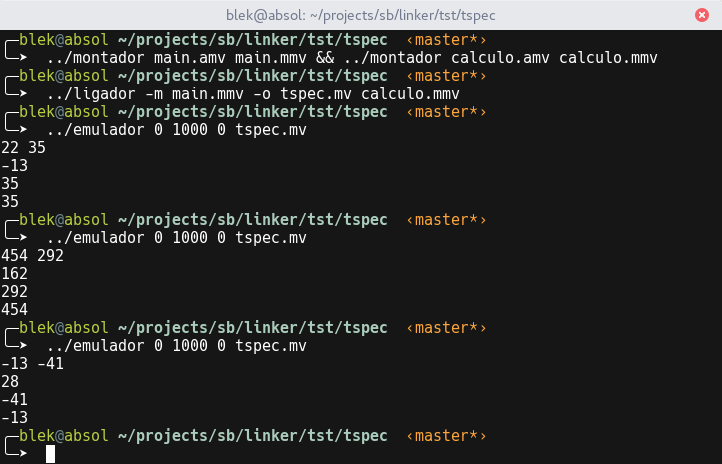
\includegraphics[scale=0.6]{imagens/tspec.png}
    \centering
    \caption{Montagem, ligação e execução do teste tspec.i.}
\end{figure}

\begin{figure}[h]
    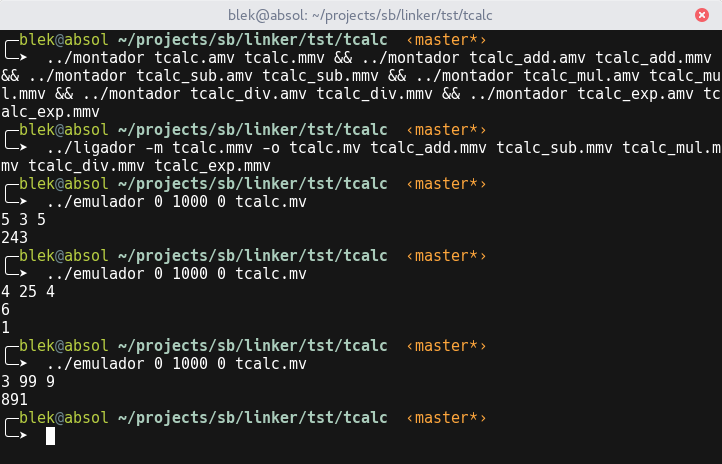
\includegraphics[scale=0.6]{imagens/tcalc.png}
    \centering
    \caption{Montagem, ligação e execução do teste tcalc.i.}
\end{figure}

\begin{figure}[h]
    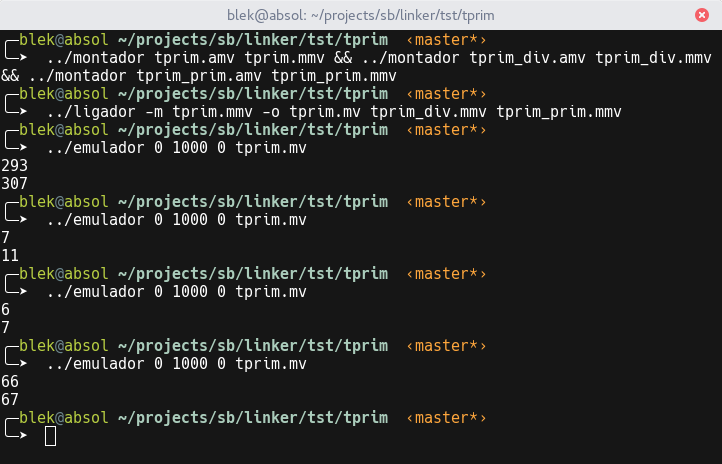
\includegraphics[scale=0.6]{imagens/tprim.png}
    \centering
    \caption{Montagem, ligação e execução do teste tprim.i.}
\end{figure}

\begin{figure}[h]
    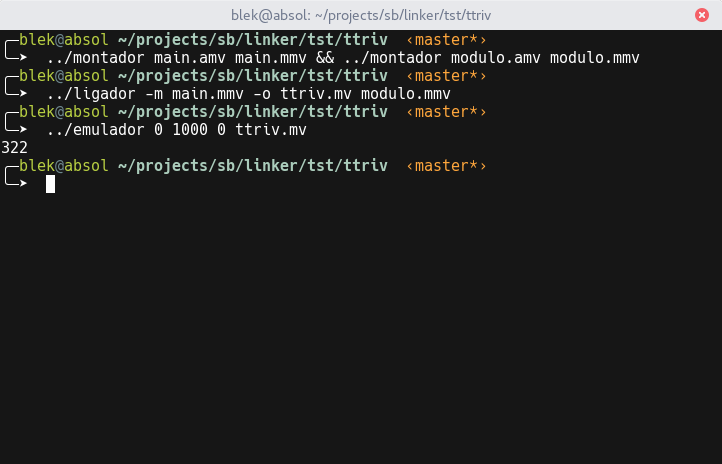
\includegraphics[scale=0.6]{imagens/ttriv.png}
    \centering
    \caption{Montagem, ligação e execução do teste ttriv.i.}
\end{figure}

\FloatBarrier

\end{document}